\documentclass[a4paper,14pt]{article}


%%% Работа с русским языком
\usepackage{cmap}					% поиск в PDF
\usepackage[T2A]{fontenc}			% кодировка
\usepackage[utf8]{inputenc}		% кодировка исходного текста
\usepackage[russian]{babel}	% локализация и переносы
%\usepackage{pscyr}
%\renewcommand{\rmdefault}{ftm}
%%% Дополнительная работа с математикой
\usepackage{amsmath,amsfonts,amssymb,amsthm,mathtools,gensymb,float} % AMS
%% Номера формул
%\mathtoolsset{showonlyrefs=true} % Показывать номера только у тех формул, на которые есть \eqref{} в тексте.
%\usepackage{leqno} % Нумерация формул слева
%\usepackage{rumathgrk1}
%% Перенос знаков в формулах (по Львовскому)
\newcommand*{\hm}[1]{#1\nobreak\discretionary{}
	{\hbox{$\mathsurround=0pt #1$}}{}}
%\usepackage{glonti}
%%% Работа с картинками
\usepackage{graphicx}  % Для вставки рисунков
\graphicspath{{images/}{images2/}}  % папки с картинками
\usepackage{wrapfig} % Обтекание рисунков текстом
\addto\captionsrussian{\def\refname{Список используемой литературы}}
%%% Работа с таблицами
\usepackage{array,tabularx,tabulary} % Дополнительная работа с таблицами
\usepackage{longtable}  % Длинные таблицы
\usepackage{multirow} % Слияние строк в таблице
%%% Теоремы
\theoremstyle{plain} % Это стиль по умолчанию, его можно не переопределять.
\newtheorem{theorem}{Теорема}[section]
\newtheorem{proposition}[theorem]{Утверждение}

\theoremstyle{definition} % "Определение"
\newtheorem{corollary}{Следствие}[theorem]
\newtheorem{problem}{Задача}[section]

\theoremstyle{remark} % "Примечание"
\newtheorem*{nonum}{Решение}
%\pagestyle{empty}
%%% Страница
\usepackage{extsizes} % Возможность сделать 14-й шрифт
\usepackage{geometry} % Простой способ задавать поля
\geometry{top=20mm}
%\geometry{bottom=35mm}
\geometry{left=25mm}
\geometry{right=20mm}
\setlength{\parindent}{1.1cm}

\usepackage{setspace} % Интерлиньяж
\onehalfspacing % Интерлиньяж 1.5
% \doublespacing % Интерлиньяж 2
%\singlespacing % Интерлиньяж 1

\usepackage{lastpage} % Узнать, сколько всего страниц в документе.
\usepackage[usenames]{color}
\usepackage{colortbl}
\renewcommand{\baselinestretch}{1.05}
\usepackage{hyperref}
\usepackage[usenames,dvipsnames,svgnames,table]{xcolor}
\hypersetup{				% Гиперссылки
	unicode=true,           % русские буквы в раздела PDF
	pdftitle={Заголовок},   % Заголовок
	pdfauthor={Автор},      % Автор
	pdfsubject={Тема},      % Тема
	pdfcreator={Создатель}, % Создатель
	pdfproducer={Производитель}, % Производитель
	pdfkeywords={keyword1} {key2} {key3}, % Ключевые слова
	colorlinks=true,       	% false: ссылки в рамках; true: цветные ссылки
	linkcolor=black,          % внутренние ссылки
	citecolor=blue,        % на библиографию
	filecolor=magenta,      % на файлы
	urlcolor=cyan           % на URL
}

\usepackage{bm}
\usepackage{tikz}
\begin{document}
% НАЧАЛО ТИТУЛЬНОГО ЛИСТА
\begin{center}
    {\textsc{Федеральное государственное бюджетное образовательное
            учреждение высшего образования
        }}\\
    {\textsc{Московский государственный университет имени М.В. Ломоносова
    }} \\
    \vspace{0.2cm}
    {\textsc{Механико - математический факультет}}\\
    \vspace{0.2cm}
    {\textsc{Кафедра прикладной механики и управления}}\\
    \hfill \break
    \begin{figure}[h!]
        \centering
        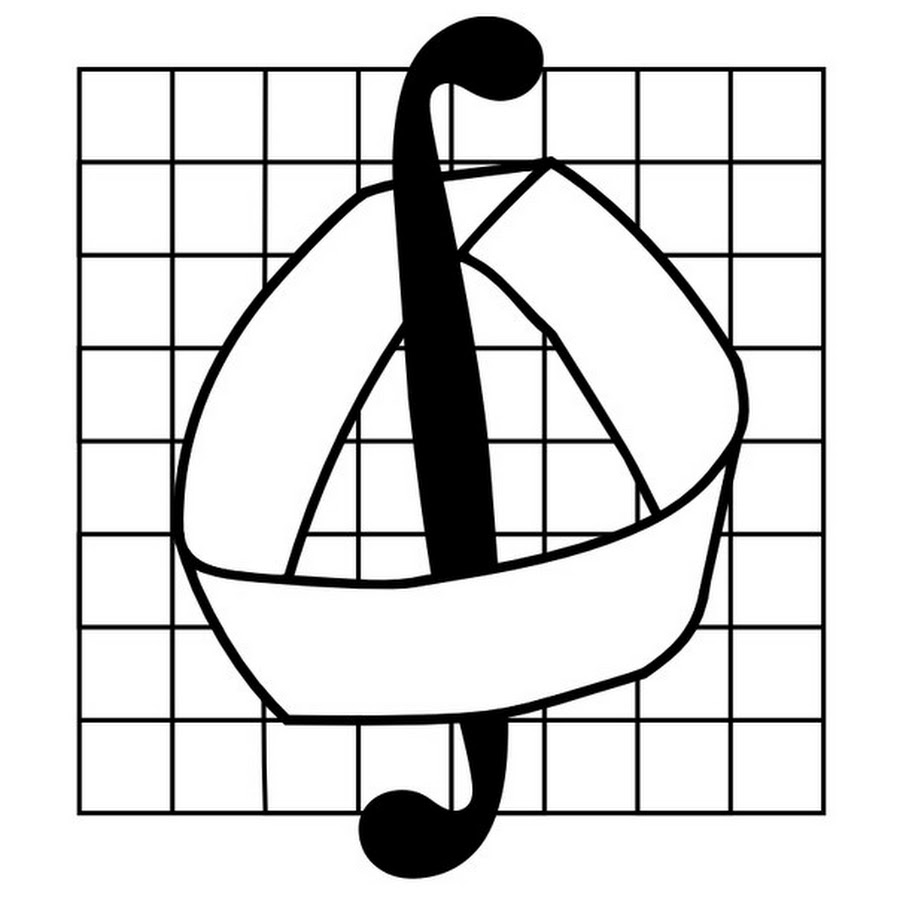
\includegraphics[width=0.30\linewidth]{emblema}
        \label{fig:emblema}
    \end{figure}
    \hfill \break
    \hfill \break
    \large{\textbf{Домашняя работа №3}\\
        \hfill \break Инерциальные навигационные системы
    }
\end{center}

\hfill \break
\hfill \break
\begin{flushright}
    {
        Выполнил: студент группы М -- 1 \\ Романов Андрей Владимирович}
\end{flushright}

\begin{flushright}
    {
        Преподаватель: д.ф.-м.н., \\ Голован Андрей Андреевич}
\end{flushright}
\hfill \break
\hfill \break
\begin{center} {Москва, 2022} \end{center}



\thispagestyle{empty} % выключаем отображение номера для этой страницы
\normalsize{
% КОНЕЦ ТИТУЛЬНОГО ЛИСТА
\newpage
\tableofcontents
\newpage

\section{Задача 1}
\textbf{Задание:}

Штатная ориентация приборного трехгранника $M s$ БИНС при установке на полу объекта такова:

\begin{itemize}
    \item ось $M x$ направлена по правому крылу;

    \item $M y$ - продольная ось;

    \item ось $M z$ - направлена вверх.

\end{itemize}
Исходный файл - IMU\_4\_8.txt , содержит колонки:

\begin{itemize}
    \item $t$ - время [сек], шкала времени - 400 гц;

    \item $A x, A y, A z$ - показания акселерометров $\left[\mathrm{m} / \mathrm{s}^{2}\right]$;

    \item $W x, W y, W z$ - показания ДУС $[\mathrm{rad} / \mathrm{s}]$.

\end{itemize}
Корпус БИНС может быть перевернут! Поэтому для решения задачи выставки потребуется перенумерация осей и смена знака так, что оставался правый приборный трехгранник.

Координаты опорной точки:
$$
    \varphi=55^{\circ}: 50^{\prime}: 30.21^{\prime \prime}, \quad h=164.78[\mathrm{~m}], \quad g^{r e f}=9.8150996\left[\mathrm{~m} / \mathrm{s}^{2}\right] .
$$
Задание:

\begin{itemize}
    \item определить интервал неподвижности.

    \item на этом интервале неподвижности определить акселерометр, ось чувствительности которого направлена вверх или вниз.

    \item при необходимости перенумеровать оси со сменой знака. Объяснить перенумерацию.

    \item определить углы курса, крена, тангажа и географической широты.

    \item представить графики накапливающихся математических ожиданий и СКО для каждого показания акселерометров и ДУС.

    \item оценить значения северного и вертикального дрейфов ДУС.

\end{itemize}
\newpage


\textbf{Решение:}

Графики исходных данных

\begin{figure}[h!]
    \centering
    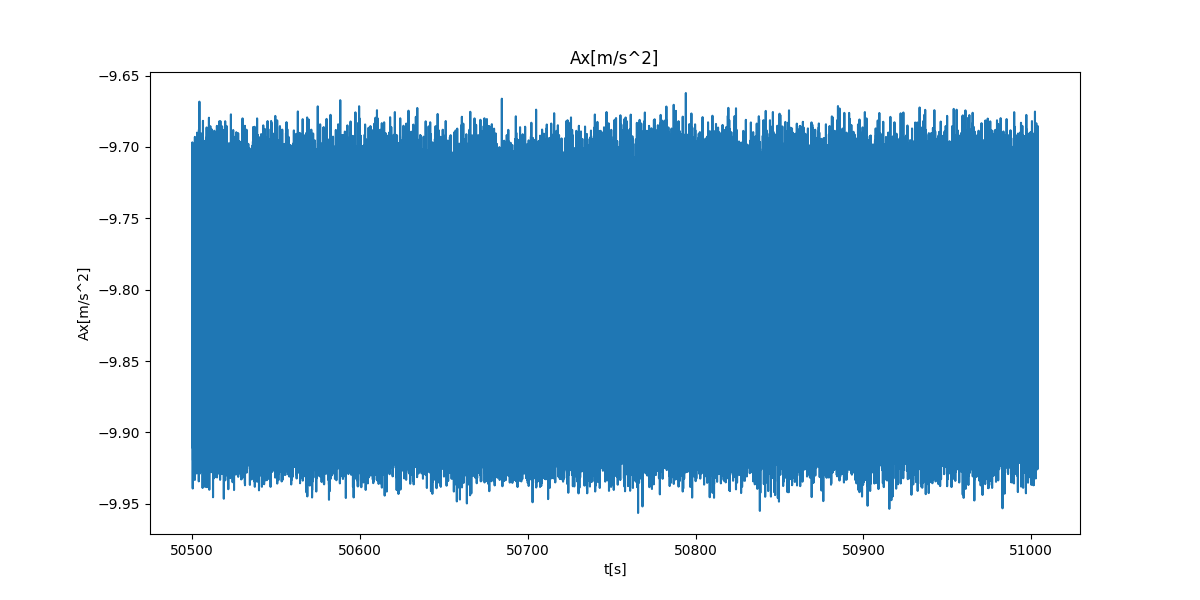
\includegraphics[width=0.99\linewidth]{Ax.png}
    \caption{Показания $Ax(m/s^2)$}
    \label{fig:ax}
\end{figure}

\begin{figure}[h!]
    \centering
    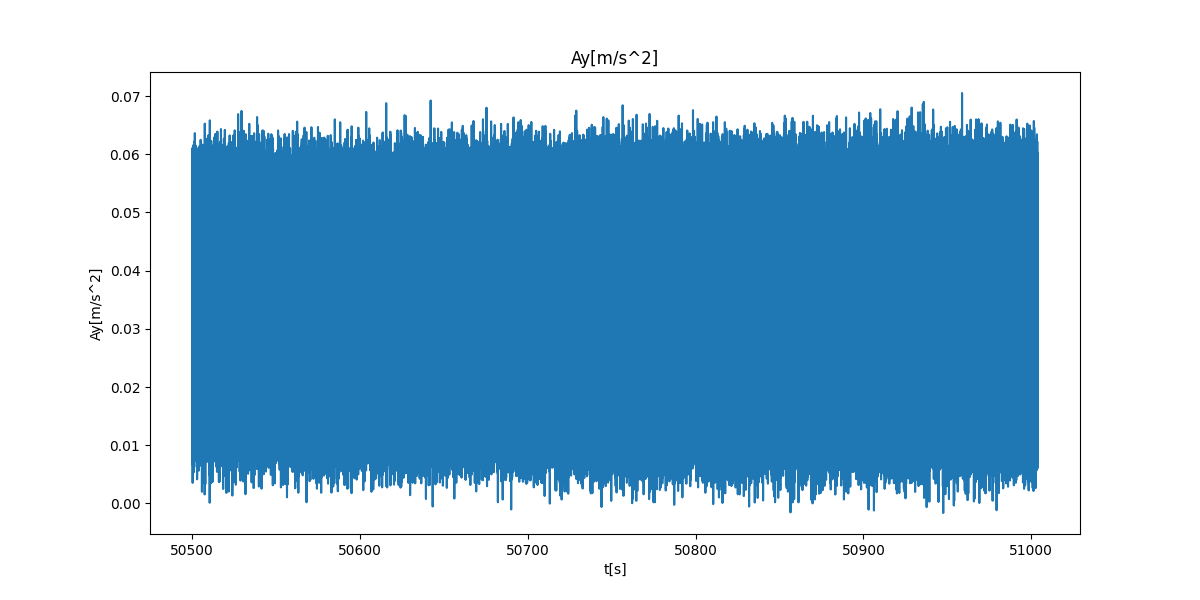
\includegraphics[width=0.99\linewidth]{Ay.png}
    \caption{Показания $Ay(m/s^2)$}
    \label{fig:ay}
\end{figure}

\begin{figure}[h!]
    \centering
    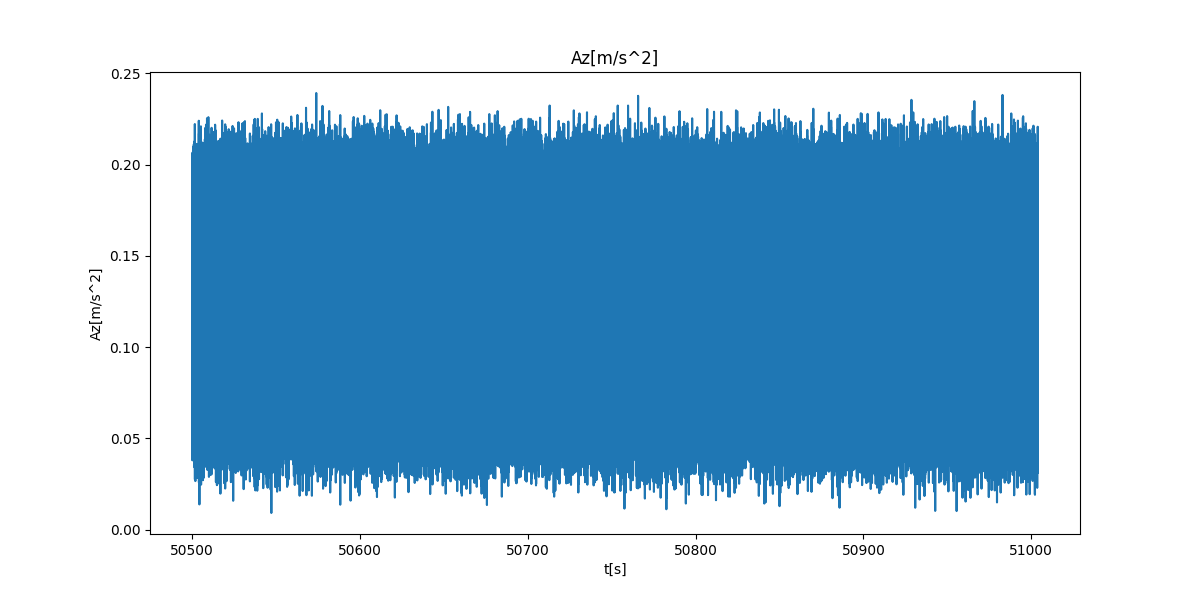
\includegraphics[width=0.99\linewidth]{Az.png}
    \caption{Показания $Az(m/s^2)$}
    \label{fig:az}
\end{figure}

\begin{figure}[h!]
    \centering
    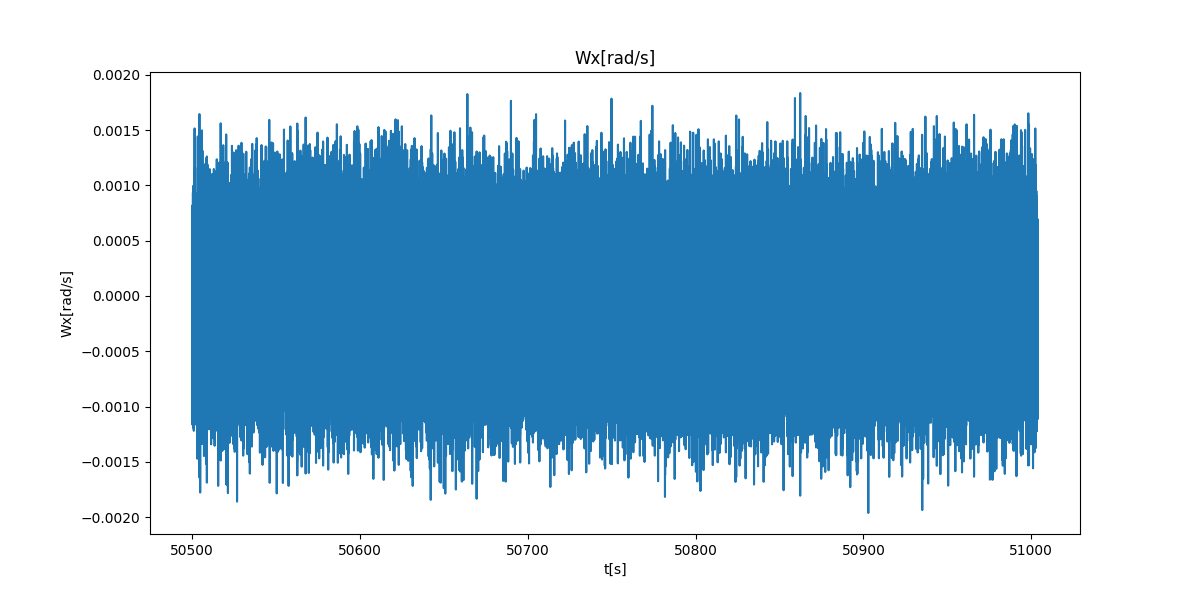
\includegraphics[width=0.99\linewidth]{Wx.png}
    \caption{Показания $Wx(rad/s)$}
    \label{fig:wx}
\end{figure}

\begin{figure}[h!]
    \centering
    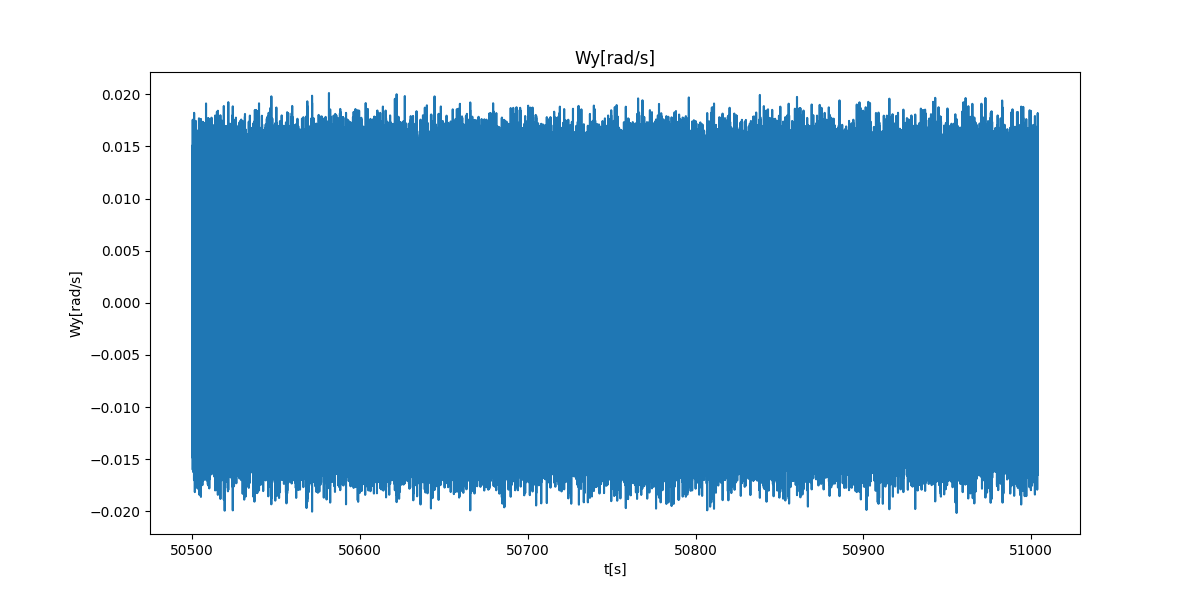
\includegraphics[width=0.99\linewidth]{Wy.png}
    \caption{Показания $Wy(rad/s)$}
    \label{fig:wy}
\end{figure}

\begin{figure}[h!]
    \centering
    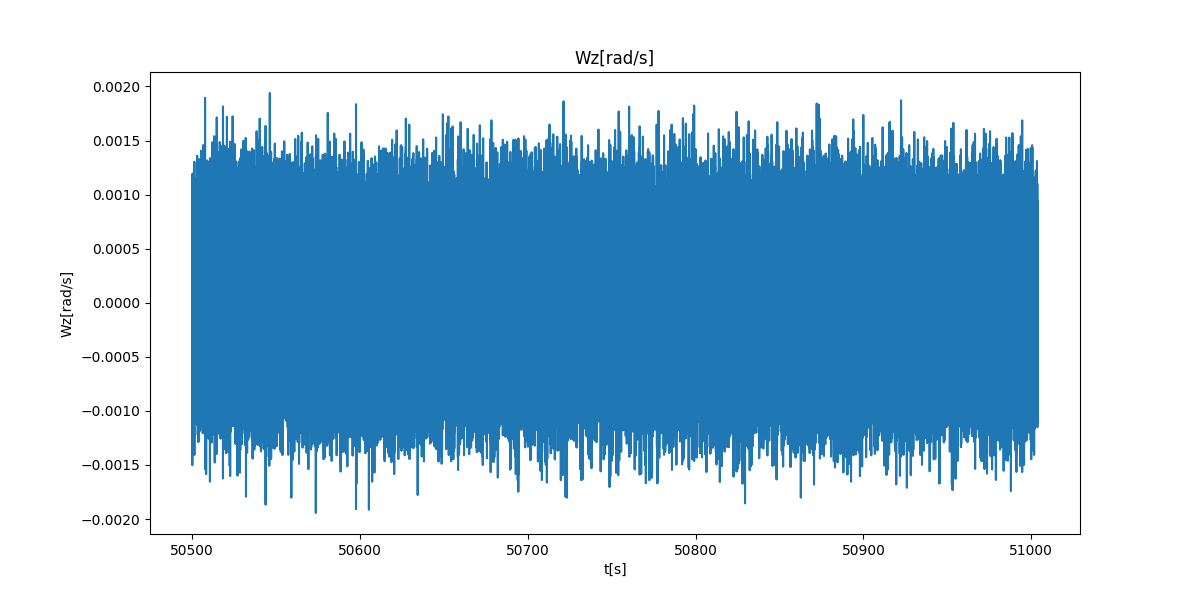
\includegraphics[width=0.99\linewidth]{Wz.png}
    \caption{Показания $Wz(rad/s)$}
    \label{fig:wz}
\end{figure}

Из графиков на рисунках \eqref{fig:ax}-\eqref{fig:wz} видно,
что нет выбросов в данных, поэтому все время наблюдения это интервал неподвижности.
Первый акселерометр $Ax$ перевернут относительно стандартной ориентации
Для того, чтобы получить измерения в стандартной ориентации перенумеруем оси
\begin{equation}\label{aksel}
    \left\{ {\begin{aligned}
                 & A_1=-A_2 , \hfill \\
                 & A_2=A_3, \hfill   \\
                 & A_3=-A_1. \hfill  \\
            \end{aligned}} \right.
\end{equation}
\begin{equation}\label{dus}
    \left\{ {\begin{aligned}
                 & W_1=-W_2, \hfill \\
                 & W_2=W_3, \hfill  \\
                 & W_3=-W_1. \hfill \\
            \end{aligned}} \right.
\end{equation}
В географических осях вектор нормальной удельной силы тяжести:
$$
    g_{x^{0}}=\left(\begin{array}{r}
            0 \\
            0 \\
            -g
        \end{array}\right)
$$
Матрица перехода от географического трехгранника к приборному
$$
    A_{s x^{0}}=\left(\begin{array}{ccc}
            \cos \psi \cos \gamma+\sin \psi \sin \vartheta \sin \gamma & -\sin \psi \cos \gamma+\cos \psi \sin \vartheta \sin \gamma & -\cos \vartheta \sin \gamma \\
            \sin \psi \cos \vartheta                                   & \cos \psi \cos \vartheta                                    & \sin \vartheta              \\
            \cos \psi \sin \gamma-\sin \psi \sin \vartheta \cos \gamma & -\sin \psi \sin \gamma-\cos \psi \sin \vartheta \cos \gamma & \cos \vartheta \cos \gamma
        \end{array}\right)
$$
Сила тяжести в $Ms$ равна
$$
    g_{s}=g\left(\begin{array}{c}
            \cos \vartheta \sin \gamma \\
            -\sin \vartheta            \\
            -\cos \vartheta \cos \gamma
        \end{array}\right)
$$
оценку показаний акселерометров найдем как среднее арифметическое всех показаний
$$
    \tilde{f}=\frac{\sum_{k=1}^{N} f^{\prime}(k)}{N}=
    \left(\begin{array}{c}
            -0.033938193479 \\
            0.123968901066  \\
            9.814114996043
        \end{array}\right),
    \quad \widetilde{f}=\left(\begin{array}{c}
            \tilde{f}_{1}     \\
            \widetilde{f}_{2} \\
            \widetilde{f}_{3}
        \end{array}\right)=g\left(\begin{array}{c}
            -\cos \vartheta \sin \gamma \\
            \sin \vartheta              \\
            \cos \vartheta \cos \gamma
        \end{array}\right)
$$
Теперь можем вычислить углы крена и тангажа
$$
    \widetilde{\vartheta}=\operatorname{atan} 2\left(\widetilde{f}_{2}, \sqrt{\widetilde{f}_{1}^{2}+\widetilde{f}_{3}^{2}}\right)=0.012630947075=0^{\circ} \ 43' \ 25.32''
$$
$$
    \widetilde{\gamma}=-\operatorname{atan} 2\left(\widetilde{f}_{1}, \widetilde{f}_{3}\right)=0.003458086461=0^{\circ} \ 11' \ 53.28''
$$
Далее рассмотрим трёхгранник $М x$ определённый как:
$$
    M x^{0} \underset{3}{\stackrel{-\psi}{\longrightarrow}} M x \underset{1}{\stackrel{\vartheta}{\longrightarrow}} \underset{2}{\stackrel{\gamma}{\longrightarrow}} M s
$$

$$
    \begin{aligned}
         & A_{x s}=A_{x s}^{(1)}(-\vartheta) A_{x s}^{(2)}(-\gamma)=\left(\begin{array}{ccc}1 & 0 & 0 \\0 & \cos (-\vartheta) & \sin (-\vartheta) \\0 & -\sin (-\vartheta) & \cos (-\vartheta)\end{array}\right)\left(\begin{array}{ccc}\cos (-\gamma) & 0 & -\sin (-\gamma) \\0 & 1 & 0 \\\sin (-\gamma) & 0 & \cos (-\gamma)\end{array}\right)= \\
         & =\left(\begin{array}{ccc}1 & 0 & 0 \\0 & \cos \vartheta & -\sin \vartheta \\0 & \sin \vartheta & \cos \vartheta\end{array}\right)\left(\begin{array}{ccc}\cos \gamma & 0 & \sin \gamma \\0 & 1 & 0 \\-\sin \gamma & 0 & \cos \gamma\end{array}\right)=\left(\begin{array}{ccc}\cos \gamma & 0 & \sin \gamma \\\sin \vartheta \sin \gamma & \cos \gamma & -\sin \vartheta \cos \gamma \\-\cos \vartheta \sin \gamma & \sin \vartheta & \cos \vartheta \cos \gamma\end{array}\right) \text {. }
    \end{aligned}
$$

$$
    \begin{aligned}
         & A_{x s}=\left(\begin{array}{ccc}0.9999940208 & 0.0000000000 & 0.0034580796
             \\0.0000436777 & 0.9999940208 & -0.0126305357 \\
             -0.0034578037     & 0.0126306112 & 0.9999142520
            \end{array}\right)
    \end{aligned}
$$
$$
    \widetilde{\omega}=\frac{\sum_{k=1}^{N} \omega^{\prime}(k)}{N}, \quad \widetilde{\omega}_{x}=A_{x s}(\widetilde{\vartheta}, \widetilde{\gamma}) \widetilde{\omega}=A_{x s}(\widetilde{\vartheta}, \widetilde{\gamma})\left(\begin{array}{c}
            \widetilde{\omega}_{1} \\
            \widetilde{\omega}_{2} \\
            \widetilde{\omega}_{3}
        \end{array}\right)
$$
$$
    \widetilde{\omega}_{x}=\left(\begin{array}{c}
            0.0000394278 \\
            0.0000109639 \\
            0.0000603351
        \end{array}\right)
$$
Угловая скорость Земли в географических осях:
$$
    u_{x^{0}}=\left(\begin{array}{c}
            0              \\
            u \cos \varphi \\
            u \sin \varphi
        \end{array}\right)
$$
$$
    \begin{aligned}
         & A_{x x_{0}}=\left(\begin{array}{ccc}\cos (-\psi) & \sin (-\psi) & 0 \\-\sin (-\psi) & \cos (-\psi) & 0 \\0 & 0 & 1\end{array}\right)=\left(\begin{array}{ccc}\cos \psi & -\sin \psi & 0 \\\sin \psi & \cos \psi & 0 \\0 & 0 & 1\end{array}\right) \\
    \end{aligned}
$$
в осях $M x$ :
$$
    u_{x}=A_{x x_{0}}(\varphi, \psi) u_{x^{0}}=\left(\begin{array}{c}
            -u \cos \varphi \sin \psi \\
            u \cos \varphi \cos \psi  \\
            u \sin \varphi
        \end{array}\right)
$$
Приравняем угловую скорость земли и усреднённые показатели ДУС в трёхграннике $M x$, получим  $\widetilde{\varphi}$ и $\widetilde{\psi}:$

$$
    \tilde{\varphi}=\operatorname{atan} 2\left(\widetilde{\omega}_{3}, \sqrt{\widetilde{\omega}_{1}^{2}+\widetilde{\omega}_{2}^{2}}\right)=0.974800431338=55^{\circ}: 51^{\prime}: 7.022^{\prime \prime},
$$
$$
    \widetilde{\psi}=-\operatorname{atan} 2\left(\widetilde{\omega}_{1}, \widetilde{\omega}_{2}\right)=-1.299573206866=-74^{\circ}: 27^{\prime}: 36.216^{\prime \prime}$$
Теперь построим графики среднего значения и квадрата СКО с небольшим отступом от начального времени в соответствии с формулами :
$$
    \begin{gathered}
        \widetilde{\mu}_{n+1}=\frac{n \widetilde{\mu}_{n}+x_{n+1}}{n+1}, \quad \widetilde{\mu}_{1}=x_{1}, \\
        \widetilde{\sigma}_{n+1}^{2}=\left(1-\frac{1}{n}\right) \widetilde{\sigma}_{n}^{2}+\left(\frac{x_{n+1}-\widetilde{\mu}_{n+1}}{n}\right)^{2}, \quad \widetilde{\sigma}_{1}^{2}=0,
    \end{gathered}
$$

\begin{figure}[h!]
    \centering
    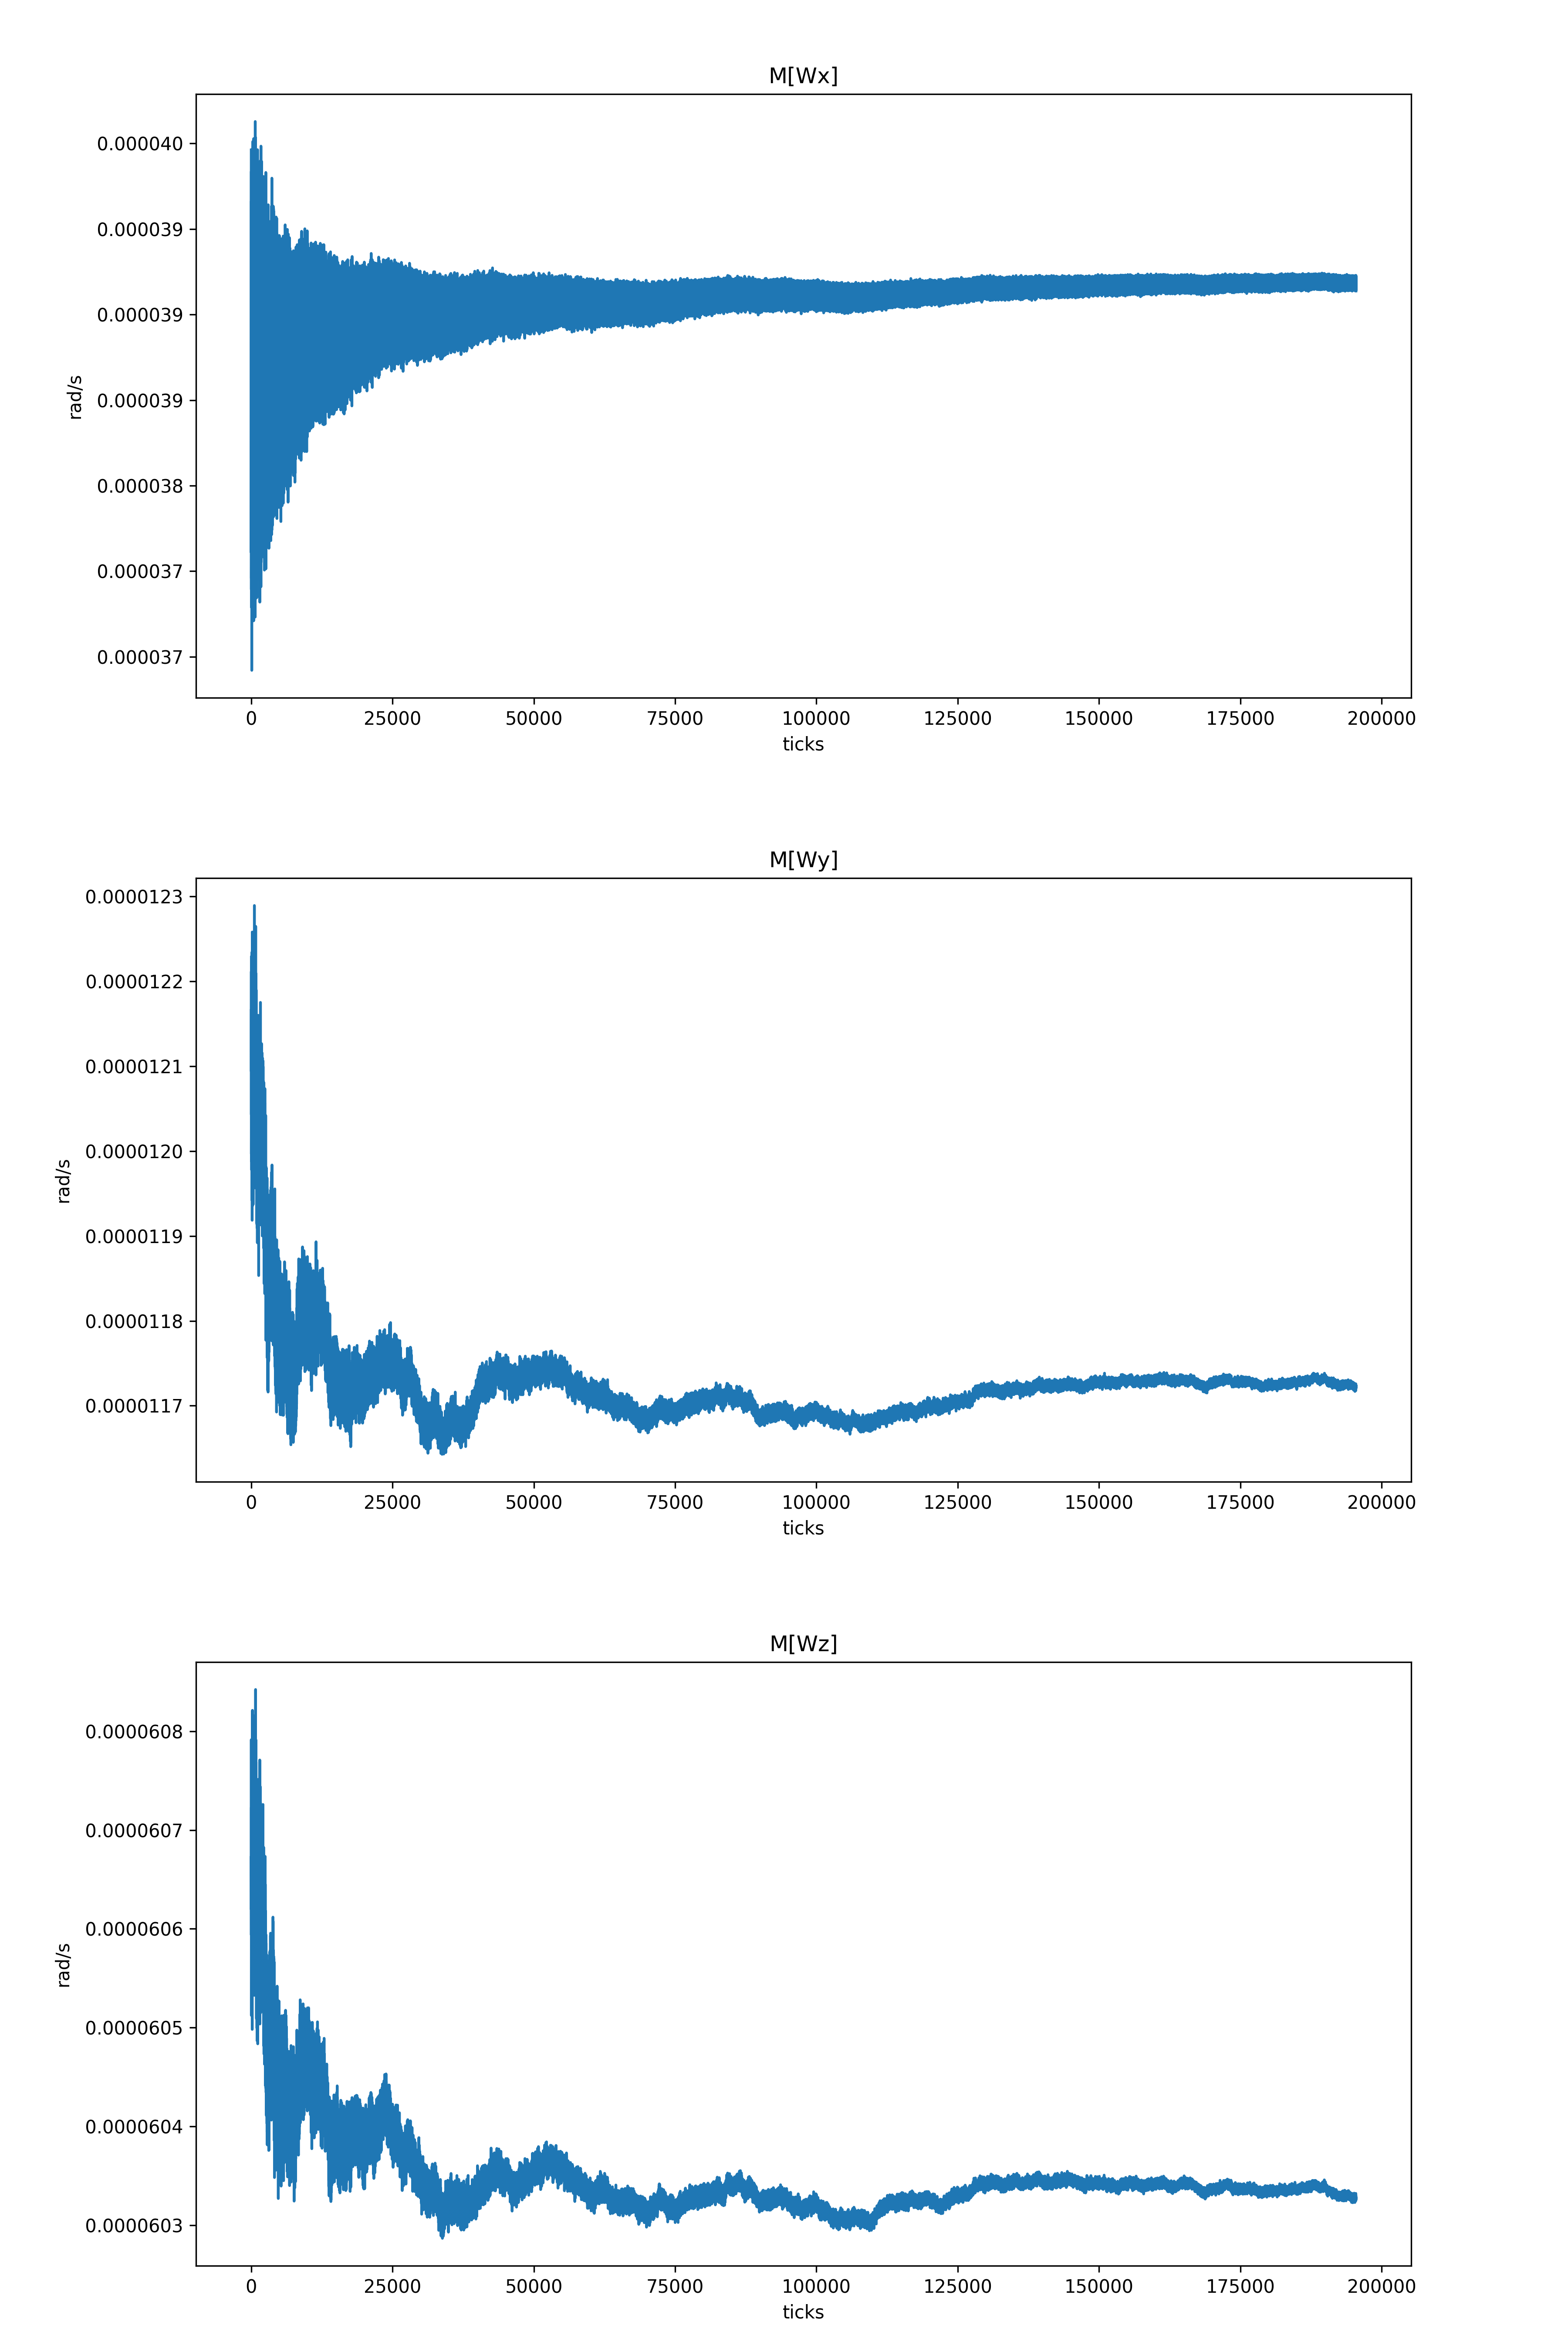
\includegraphics[width=0.99\linewidth]{FullW.png}
    \caption{ График $\widetilde{f}$}
    \label{fig:ma}
\end{figure}

\begin{figure}[h!]
    \centering
    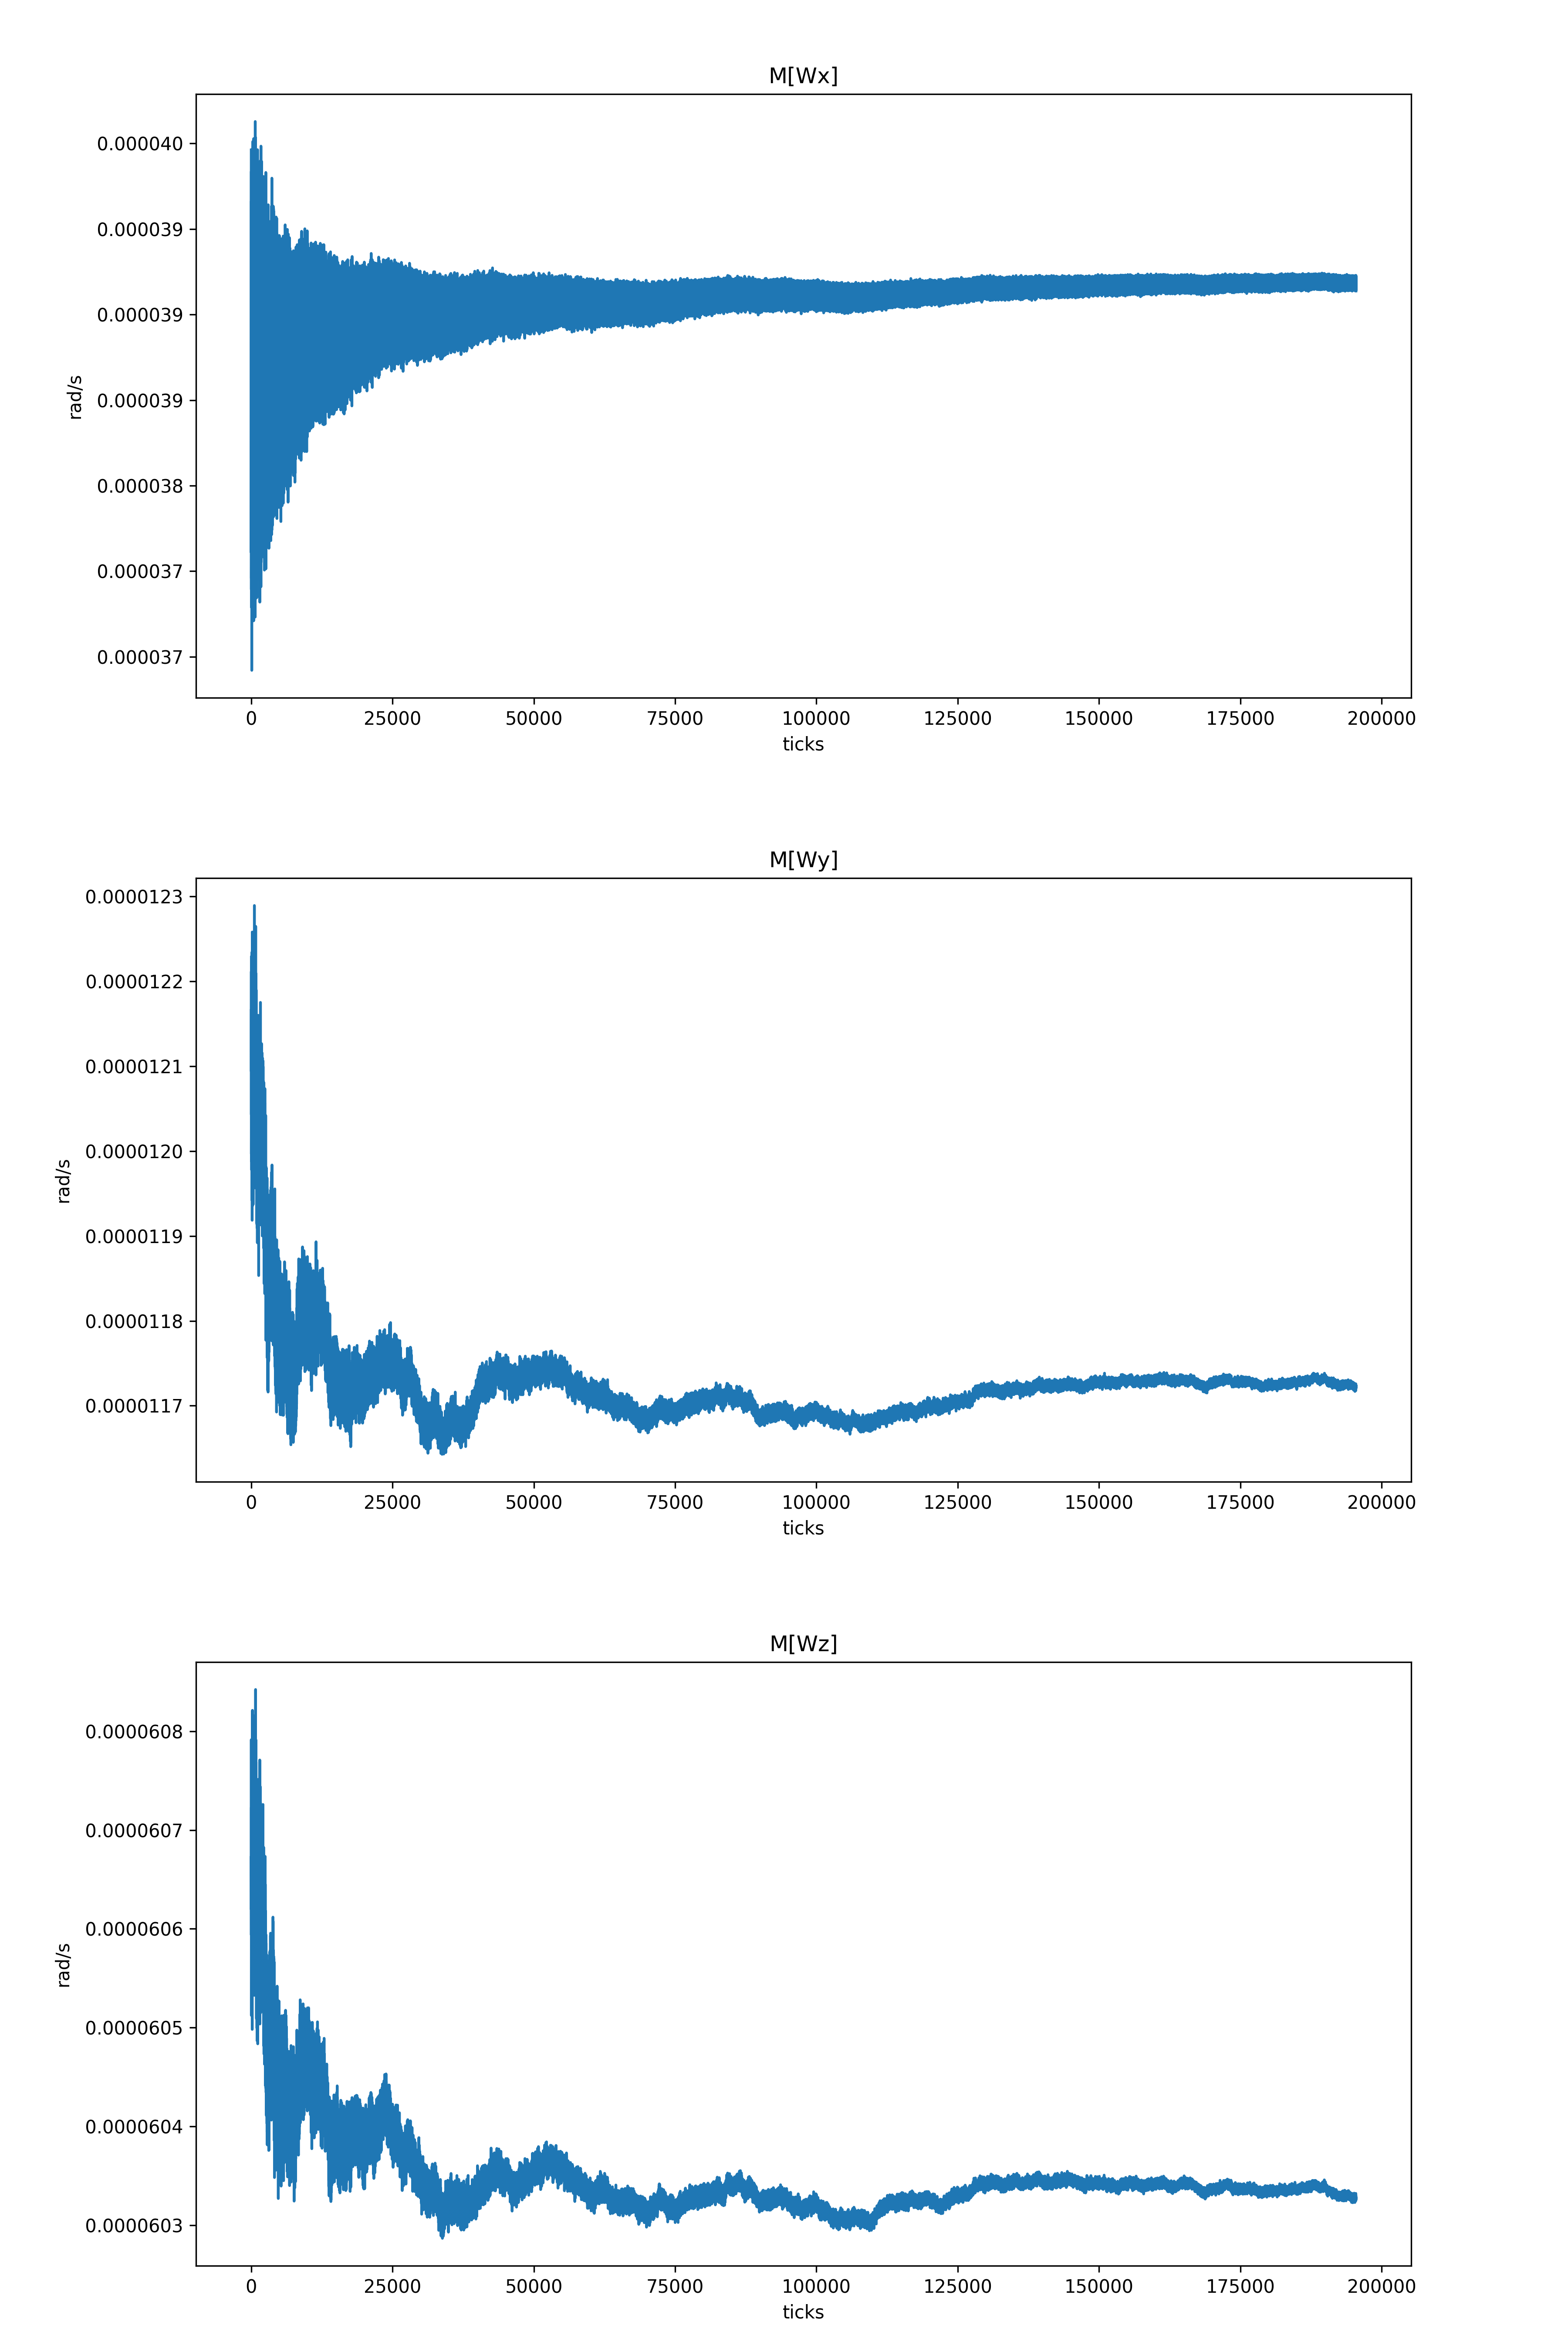
\includegraphics[width=0.99\linewidth]{FullW.png}
    \caption{ График $\widetilde{w}$}
    \label{fig:mw}
\end{figure}

Как видно из Рис.8-11 качество входных измерений достаточно хорошее: присутствующие шумы ведут себя очень похоже на математический белый шум, за счёт этого средние значения показания акселерометров и ДУС быстро стабилизируются. Также можно сделать вывод, что для решения задачи выставки нам бы хватило и например одной пятой интервала измерений.

Осталась оценить значения северного $\left(\widetilde{\nu}_{N}\right)$ и вертикального дрейфа $\left(\widetilde{\nu}_{U P}\right)$ ДУС как:
$$
    \left(\begin{array}{c}
            0                   \\
            \widetilde{\nu}_{N} \\
            \widetilde{\nu}_{U P}
        \end{array}\right)=\omega_{x^{0}}-\widetilde{\omega}_{x^{0}}=\omega_{x^{0}}-A_{x^{0} s}(\widetilde{\psi}, \widetilde{\vartheta}, \widetilde{\gamma}) \widetilde{\omega}
$$
где $\omega_{x^{0}}$ определяется из формулы $(11)$, а матрица ориентации географического трёхгранника относительно приборного:

$$
    A_{x^{0} s}=\left(\begin{array}{ccc}
            \cos \psi \cos \gamma+\sin \psi \sin \vartheta \sin \gamma  & \sin \psi \cos \vartheta & \cos \psi \sin \gamma-\sin \psi \sin \vartheta \cos \gamma  \\
            -\sin \psi \cos \gamma+\cos \psi \sin \vartheta \sin \gamma & \cos \psi \cos \vartheta & -\sin \psi \sin \gamma-\cos \psi \sin \vartheta \cos \gamma \\
            -\cos \vartheta \sin \gamma                                 & \sin \vartheta           & \cos \vartheta \cos \gamma
        \end{array}\right)
$$

Промежуточно вычислим:
$$
    \widetilde{\omega}_{x^{0}}=A_{x^{0} s}(\widetilde{\psi}, \widetilde{\vartheta}, \widetilde{\gamma}) \widetilde{\omega}_{s}=\left(\begin{array}{c}
            0            \\
            0.0000409236 \\
            0.0000603351
        \end{array}\right)=\left(\begin{array}{c}
            0             \\
            \tilde{u}_{N} \\
            \widetilde{u}_{U P}
        \end{array}\right)
$$

$$
    \widetilde{\nu}_{N}=u \cos \widetilde{\varphi}-\widetilde{u}_{N}=0.000000009507=0^{\circ}: 0^{\prime}: 0.00196096^{\prime \prime}\left(\frac{1}{\text { чac }}\right)
$$
$$
    \widetilde{\nu}_{U P}=u \sin \widetilde{\varphi}-\widetilde{u}_{U P}=0.000000013675=0^{\circ}: 0^{\prime}: 0.00282067^{\prime \prime}\left(\frac{1}{\text { час }}\right)
$$.
\end{document}